% -*- root: ../thesis.tex -*-

\chapter[Introduction]{Introduction}
\label{ch:intro}
\label{sec:intro:abs}

% \section{From actor \emph{modelling} to actor \emph{programming}}

Object-oriented programming~\cite{booch1982object,meyer1988object} has been of one the dominant paradigms for software engineering in the past three decades.
SIMULA 67~\cite{Dahl:1968:simula} introduced notions of classes, subclasses, and virtual procedures.
In the main block of a program, objects are created, then their procedures are called.
One object interacts with another object using the notion of a method.
Method invocations are \emph{blocking}; i.e. the caller object waits until it receives the result of the method call from the callee object.
This model of interaction was not the intention of the pioneers of the paradigm.
Object interactions were meant to be \emph{messages} among objects and objects behaved as autonomous entities possibly on remote locations on a network; Alan Kay clarified later~\cite{alank1,alank2}. 
On the contrary, almost all the object-oriented languages at hand have followed the blocking and synchronous model of messaging. 
The above definition of object-oriented programming has inspired another model of computation: actor model.

One of the fundamental elements of actor model~\cite{actors:agha,agha97} is \emph{asynchronous} message passing.
In this approach, interactions between objects are modelled as \emph{non-blocking} messages.
One object, the sender, communicates a message to the other object, the receiver.
At the receiver side, a message eventually leads to a method invocation (in the object-oriented paradigm) or a function call (in the functional paradigm).
Actor model features location transparency; i.e. the physical location of objects is not visible to other objects.
A system is composed of objects that communicate through messages.

A considerable amount of research has been carried out to mix object-oriented programming languages with the actor model~\cite{philippsen2000survey}. 
Language extensions, libraries, and even new programming languages are the natural outcomes of such research.
For example, \cite{actor_frameworks_jvm:agha} presents a comparative analysis of such research for Java and JVM languages.

The rapid increase of computational power added a new aspect to create a triangle: object orientation, actor model, and \emph{concurrency}.
Concurrency makes it harder to verify programs in terms of correctness of runtime behavior~\cite{Herlihy:1990:linear,johnsen:history,agha:predictive:safety}. 
The main and foremost challenge is how to combine concurrency with object-oriented programming.
Concurrency brings about two aspects in combination of object orientation: \emph{communication} and \emph{execution}.

In a concurrent setting, coroutines~\cite{conway1963design,taocp:knuth} enable interactions with collaborative preemption.
A coroutine allows multiple entry points for suspending and resuming execution at certain locations.
An instance of a coroutine spawns a new process with its own state.
A coroutine may \emph{yield} to another coroutine;
there's no \emph{return} statement in a coroutine but transfer of control from one to another without returning.
The yield relation is symmetric and not similar to that of caller-callee type.
A coroutine has explicit ability to transfer control to another coroutine.
This fundamental property makes compositional concurrency of coroutines straightforward.
Coroutines are not originally established in object-oriented principles.
Object orientation is based on caller-callee interaction which is asymmetric.
Caller invokes a method in the callee and waits until the \emph{return} occurs in the method of the callee.
Object orientation focuses on an object-view with caller-callee interaction  whereas coroutines focus on process-view with transfer of control.

In a concurrent setting with objects, multi-threading has been a dominant approach to provide an object-oriented concurrency model.
A thread holds a single stack of synchronous method calls.
Execution in a thread is sequential.
The stack has a starting location (i.e. start of invocation) and a finish location (i.e. the return point).
In a caller-callee setting, an object might call methods from other objects.
With objects running in different threads, the execution of methods are interleaved in uncontrollable threads. 
Future values are used to hold the eventual return value of a method in the caller site.
The unit of interleaving in coroutines is coarse whereas multi-threading is based on implicit scheduling of method invocations.
In addition, interactions in both coroutines and multi-threading are blocking and synchronous.
In contrast, actor model relies on asynchronous communication as one of its core elements.

In actor model, every communication is asynchronous.
The unit of communication is a \emph{message}.
A queue of messages (inbox) is utilized among actors in the system.
The notion of a message is not bound by a specific definition or object interface.
When an actor receives a message, it may use pattern matching techniques to determine the content of the message.
When the actor completes the processing of a message, it may decide to reply to the message by sending another message.
On the other hand, actor model works based on run-to-completion style of execution.
When a message is being processed, an actor cannot be preempted or intentially yield to allow other actors in the system to make progress.

A question naturally rises: how to bring coroutine execution (co-operative scheduling) to an object-oriented setting with asynchronous communication with binding to object interfaces for the messages?
There are a few modelling languages that focus on the question.

Rebeca~\cite{sirjani2002simulation,sirjani2004formal,sirjani2007rebeca} is a modelling language for reactive and concurrent systems. 
In Rebeca, a number of reactive objects (\emph{rebecs}) interact at runtime.
Rebecs interactions is based on asynchronous message passing that leads to a method invocation.
In Rebeca, each rebec has a unique thread of control and an unbounded queue of messages.
Rebeca uses run-to-completion execution and does not support future values.

ABS~\cite{johnsen2012abs,hahnlehjlssw11} is a modelling language for concurrent objects and distributed systems.
ABS uses asynchronous communication among objects.
A message in ABS is bound to a method invocation;
this defines the interface of the sent messages.
In addition, ABS supports future values in its asynchronous communication.
ABS introduces \bfjtt{release} semantics that is based on co-operative scheduling of objects; 
i.e. similar to that of \emph{yield} in coroutines~\cite{creol:broch:owe}.
ABS semantics is completely expressed in structural operational semantics~\cite{plotkin:sos}.
This allows ABS models to take advantage of various verification methods and static analysis techniques.
% 
Co-operative scheduling in ABS has been additionally extended for real-time scheduling with priorities and time constraints~\cite{bjork2013:rtabs,johnsen2012modeling}.
All the above characteristics make the ABS language an attractive choice if it
can be used as a programming language at industrial and business scale.
ABS has mainly developed as a modelling language.

Considering the mainstream programming languages
\footnote{\url{http://www.tiobe.com/index.php/content/paperinfo/tpci/index.html}}, Java~\cite{gosling2000java} is one of the most commonly-used.
Since Java 1.5 and the rise of the concurrency API in Java JSR-166~\cite{jsr166}, substantial effort focus on how concurrency can be improved in Java.
However, not all the development on Java libraries and frameworks are based on a rigorous formal semantics. 
Therefore, this gives rise to issues and challenges in terms of correctness, semantic preservation, and reasoning.
In addition, the Java language specification (JLS)~\cite{gosling2000java} clearly reveals that Java language is not comptabile and ready to be extended as a functional language that supports algebraic data types.
This has been the focus of research and development to extend Java to a functional language~\cite{odersky1997pizza,henkel2003discovering,nystrom2003polyglot,bracha1998making}.
Scala~\cite{odersky2004scala} is a result of such relevant research. It is a dynamic, functional, and object-oriented language on JVM.

One core challenge is how to create a mapping of coroutines to multi-threading in Java.
Supporting coroutines in Java can be mostly classified in two major categories.
One category relies a \emph{modified} JVM platform (e.g. Da Vinci JVM) in the implementation of thread stack and state such as \cite{Stadler:2009:LCJ:1596655.1596679}, \cite{Stadler:2010:ECJ:1852761.1852765} and \cite{Liu:2006:II:1111320.1111063}.
Other category involves libraries such as Commons Javaflow\footnote{\url{http://commons.apache.org/sandbox/commons-javaflow/}} or Coroutines\footnote{\url{https://github.com/offbynull/coroutines}} that utilize byte-code modification~\cite{dahm1999byte} at runtime in JVM.
In this research, we did not intend to use any of the two above approaches.
Custom or modified JVM platform implementations are not mainstream and not officially supported by Java team.
Research and development on a modified JVM requires explicit and periodic maintenance and upgrade effort.
Moreover, since byte-code modification changes the byte-code of a running program or inserts new byte-code into JVM at runtime, it makes reasoning and correctness analysis/verification more complicated~\cite{leroy2001java,leroy2003java}.
We rely on the mainstream JVM platform released by Java team at Oracle; in addition, we do not use byte-code engineering.

Since a thread owns a single stack, a straightforward approach is to map every invocation (entry point) in a coroutine to a new thread in Java~\cite{SchaferP10,schafer2010programming}. 
This mapping unsurprisingly leads to a poor performance;
the number of threads is not scalable at runtime based on resource limitations in JVM when the number of object increase (cf. Chapter~\ref{ch:p01:ch01}).
Therefore, it is reasonable to use a pool of threads (JSR-166~\cite{jsr166}) to direct the execution of all method invocations (messages). 
However, to deploy a message onto a thread for execution, the message is required to be abstracted in a generic way.
We utilize Java~8 features (JSR 335~\cite{jsr335} and JSR 292~\cite{jsr292:invokedyn}) to abstract a message as a data structure expressed in a lambda expression (cf. Chapter~\ref{ch:p02:ch01}).

The core contributions of this thesis target at the intersection of object 
orientation, actor model, and concurrency.
We choose Java as the main programming language and as one of the mainstream 
object-oriented languages. 
We formalize a subset of Java and its concurrency API~\cite{jsr166} to 
facilitate formal verification and reasoning about it.
We create an abstract mapping from a concurrent-object modelling language, 
ABS~\cite{johnsen2012abs}, to programming semantics of Java concurrency (cf. Chapter~\ref{ch:p01:ch02}). 
We provide the formal semantics of the mapping and runtime properties of 
the concurrency layer including deadlines and scheduling policies (cf. Chapter~\ref{ch:p01:ch01}).
We provide an implementation of ABS concurrency layer as a Java API library 
and framework utilizing the latest langauge additions 
in Java 8~\cite{jsr335:lambda:translation} (cf. Chapter~\ref{ch:p02:ch01}).
We design and implement a runtime monitoring framework, JMSeq, to verify the
sequenced execution of methods through code annotatinon in JVM (cf. Chapter~\ref{ch:p03:ch02}). 
In addition, we design a large-scale monitoring system as a real-world 
application; the monitoring system is built with actors and ABS concurrency 
with formal semantics of ABS composed with schedulability 
analysis~\cite{fersman2007task} (cf. Chapter~\ref{ch:p03:ch01}).

\section{Objectives and Architecture}
\label{sec:intro:arch:crit}

In this section, we present a high-level overview of design goals that we pursue in this research. 

\paragraph{Polyglot Programming}
With the rise of distributed computing challenges, software engineering practice has turned to methods that combine multiple programming languages and models to complete a task. 
In this approach, different languages with different focus and abstractions contribute to the same problem statement in different layers. 
Polyglot programming essentially enables software practice to apply the \emph{right} language in the appropriate layer of the problem statement. 
In this research, we aim to deliver ABS semantics and features in a polyglot approach. 
The programmer develops models with ABS that \emph{partially} take advantage of the target language features (e.g. from Java).
This approach is also referred to as \emph{Foreign Function Interface} in the context of ABS modelling.

\begin{lstlisting}[float=h,language=Java,caption=Using Java in ABS,label=lst:abs:java]
java.util.List<String> params = new java.util.ArrayList<>();    // Java
myObj ! doSomething(params);                                    // ABS
\end{lstlisting}

Listing~\ref{lst:abs:java} shows a snippet of ABS code that uses \jtt{java.util.ArrayList} as a data strucuture.
Ideally in ABS, the programmer is able to directly use the libraries and API from Java.
This removes the necessity to redundantly repeat definition of common data structures and API at ABS.

\paragraph{Scalability} 
Asynchronous message passing in ABS is a fit for distributed systems.
In such systems, the number of messsages delivered among actors in the 
environment is not predictable at runtime.
The goal is to ensure the actor system scales in performance with least 
influence from the number of asynchronous messages delivered in the system.

\paragraph{Modularity} 
We approach ABS modelling and development with a component-based or modular 
software engineering practices.
The scope of the research spans to a number of layers around ABS language:

\begin{itemize}
\item \emph{Compiling ABS to a target programming language}
One first objective is to compile an ABS model to a target programming language.
Target languages potentially include mainstream programming languages such as
Java, Erlang, Haskell, and Scala.
Thus, the ABS programmer should be able to use an ABS compiler to compile
their ABS models to the target languages.
We propose a new architecture for ABS tool-set and engineering that enables
different programming language utilize the same architecture.
\item \emph{Using ABS concurrency as an API in an existing programming language}
The ABS language is precisely expressed with structural operational semantics~\cite{johnsen2012abs} in addition to its syntax definition.
The semantics of ABS can be delivered in a programming language
as Application Programming Interface (API) as long as the programming language provides sufficient constructs to respect ABS language semantics.
In addition, such ABS programming API should be \emph{verifiable}.
If an ABS mapping to a programming API is provided, a programmer is able to
take advantage of ABS semantics without directly programming in ABS.
Such capability from ABS enables industry users of mainstream languages to
model their systems in ABS semantics using their programming languages and
platforms.
\item \emph{Modelling in ABS}
ABS language provides a rigorous semantics to model concurrent
and distributed systems.
For practical reasons, the user (that can be a programmer, an analysist, or a researcher) 
desires to have access to a tool-set and IDE that allows working with ABS 
models in a user-friendly way.
The ABS IDE and tool-set developers should be able to easily reuse and compose
over existing modules and components.
\end{itemize}

This approach yields to a modular architecture presented in 
Figure~\ref{fig:arch}.

\begin{figure}[t]
\centering
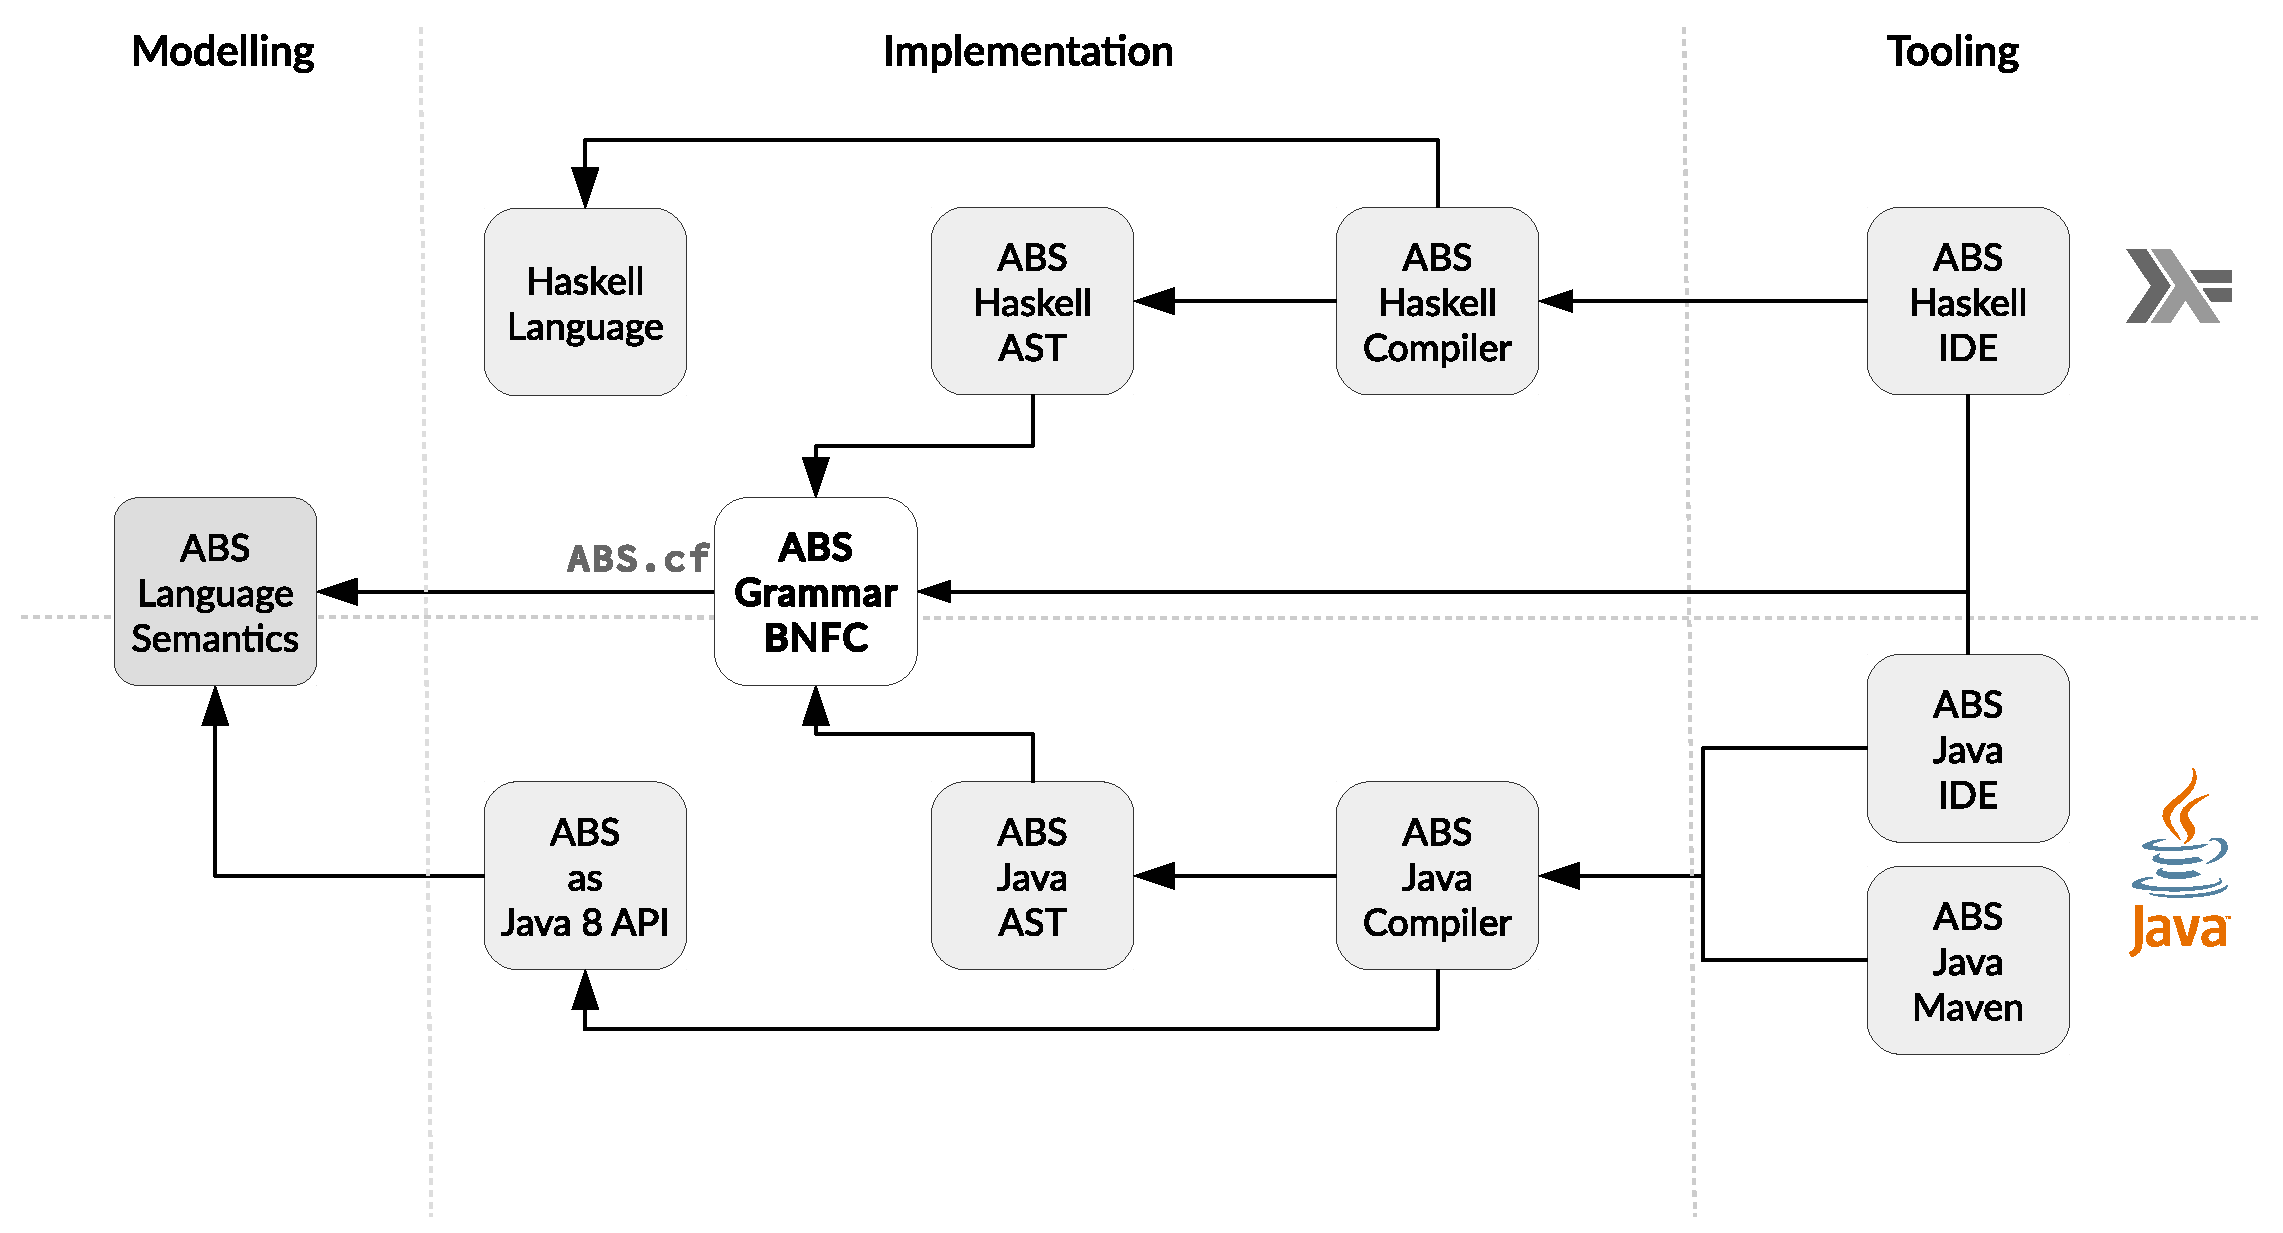
\includegraphics[scale=0.3]{../figs/Arch.eps}
\caption[General Architecture]{General Architecture of ABS API and Java Language Backend}
\label{fig:arch}
\end{figure}

\section{Literature Overview}
\label{sec:intro:rel}

We discuss a brief overview of related work in the context of programming languages, actor model, and concurrency.
We divide the overview in two levels; one is at the level of the programming languages and the other is for the external (third-party) libraries developed for programming languages.

\subsection{Programming Languages}
\label{sec:intro:proglangs}

In this section, we briefly provide an overview of the programming languages that have targetted similar problem statements.
Various programming languages, in the past decade, have emerged to provide an actor-based model of asynchronous message passing~\cite{philippsen2000survey}.
We observe different classes of actor model and concurrent model of 
programming.
Table~\ref{tbl:actor:pl} presents a summary.

\begin{description}
\item[First-Class Citizen]
Languages in which the actor model is by-design part of the syntax and 
semantics of the language.
Pony~\cite{ponylang,ClebschD13} targets high-performance 
computing using actor models and shared memory. 
When actor model is part of the design of a language, formal verification
and correctness of actor semantics at runtime yields naturally from the 
language semantics at runtime.
\item[Implicit By Design]
refers to the type that there is no explicit notion of actor models in the language syntax or semantics.
However, the programming language provides fundamental constructs for concurrency and asynchronous message passing.
Thus, it becomes an easy task in this kind of programming language to create an abstraction to support the actor model by coding.
\item[External Library]
refers to the type of programming languages for which actor model support is provided by an external library developed for the language.
\end{description}


\begin{table}[t]
\centering
\begin{tabular}{lll}
\textsfb{Language} & \textsfb{Abstraction} & \textsfb{Type} 
\\ \toprule
Erlang\cite{erlang:armstrong,erlang:actor} & Process & Implicit By Design 
\\ \midrule
Elixir\cite{elixir,elixir:actor} & Agent & Implicit By Design 
\\ \midrule
Haskell\cite{con_haskell:wiki} & forkIO \& MVars & Implicit By Design 
\\ \midrule
Go\cite{go:actor} & Goroutine & Implicit By Design 
\\ \midrule
Rust\cite{rust:2014,rust:actor} & Send \& Sync & Implicit By Design 
\\ \midrule
Scala\cite{haller09tcs} & Akka Actors
\footnote{Scala 2.11.0 adopts Akka as default actor model implementation: \url{http://docs.scala-lang.org/overviews/core/actors-migration-guide.html}}
& External Library 
\\ \bottomrule
\end{tabular}
\caption{Actor Model Support in Programming Languages}
\label{tbl:actor:pl}
\end{table}

\subsection{Frameworks and Libraries}
\label{sec:intro:libs}

Since programming languages faced challenges to provide the necessary syntax 
and semantics for actor model and concurrency at the level of the language, 
many libraries and frameworks aim to fill this gap 
Table~\ref{tbl:actor:libs} presents a summary.
We observe that the more the language itself is close to the actor model 
semantics, the less external libraries and frameworks target this gap. 
In the following, we briefly enumerate frameworks
\footnote{A more comprehensive list can be obtained at \cite{KarmaniSA09} and  \url{https://en.wikipedia.org/wiki/Actor_model\#Programming_with_Actors}}
and libraries for Java.

\begin{table}[t]
\centering
\begin{tabular}{lll}
\textsfb{Library} & \textsfb{Technique} & \textsfb{JVM Language} 
\\ \toprule
Killim\cite{srinivasan2008kilim,kilim} & Byte-Code Modification & Java 
\\ \midrule
Quasar\cite{quasar} & Byte-Code Modification, Java~8 & Clojure, Java 
\\ \midrule
Akka\cite{akka,scala:actors:ordersky} & Scala Byte-Code on JVM & Scala, Java 
\\ \bottomrule
\end{tabular}
\caption{Actor programming libraries in Java}
\label{tbl:actor:libs}
\end{table}

One of the main techniques used in libraries to deliver actor programming in 
Java is byte-code engineering~\cite{dahm1999byte,bruneton2002asm,asm}.
Byte-code engineering modifies the generated byte-code for compiled classes in 
Java either during compilation or at runtime.
Although, this technique is commonly used and argued to provide better 
performance optimization~\cite{vallee1999soot}, it introduces other challenges 
regarding the verification of the running 
byte-code~\cite{leroy2001java,leroy2003java}.

\section{Organization and Contributions}
\label{sec:intro:contribs}

Based on the problem statement and approach taken in this research, 
Table~\ref{tbl:thesis} summarizes the structure of this text:

\begin{table}[h]
\centering
\begin{tabular}{p{7cm}p{3cm}p{3cm}}
\textsfb{Topic} & \textsfb{Part} & \textsfb{Chapter/Section}
\\ \toprule
{Formalization of the mapping from ABS to Java including the operational semantics and ABS co-operative scheduling in Java} & Programming Model (Part~\ref{p:model}) & Chapter~\ref{ch:p01:ch01} and \ref{ch:p01:ch02}
\\ \midrule
Design and implementation of ABS concurrency layer in Java & Implementation (Part~\ref{p:impl}) & Chapter~\ref{ch:p02:ch01} and \ref{ch:p02:ch02}
\\ \midrule 
Monitoring method call sequences using annotations & Application (Part~\ref{p:app}) & Chapter~\ref{ch:p03:ch02}
\\ \midrule
Design and implementation of a massive-scale monitoring system based on ABS API in Java & Application (Part~\ref{p:app}) & Chapter~\ref{ch:p03:ch01}
\\ \bottomrule 
\end{tabular}
\caption{Thesis Contributions Summary}
\label{tbl:thesis}
\end{table}

In addition, Table~\ref{tbl:papers} summarizes the conference and journal 
publications as a result of this research:

\begin{table}[h]
\centering
\begin{tabular}{p{7cm}p{5cm}p{1cm}}
\textsfb{Topic} & \textsfb{Proceedings / Journal} & \textsfb{Year}   
\\ \toprule
Programming and Deployment of Active Objects with Application-Level Scheduling & ACM SAC 2012, Pages 1883--1888 & 2012 
\\ \midrule
The Future of a Missed Deadline & COORD 2013, Pages 181--195 & 2013 
\\ \midrule
Monitoring Method Call Sequences using Annotations & Journal of Science of Computer Programming, 2014, Volume 94, Part 3, Pages 362--378 & 2014 
\\ \midrule
Programming with actors in Java~8 & ISoLA 2014, Pages 37--53 & 2014 
\\ \midrule
Formal verification of service level agreements through distributed monitoring & ESOCC 2015, Pages 125--140 & 2015
\\ \bottomrule
\end{tabular}
\caption{Actors At Work -- Conference and Journal Publications}
\label{tbl:papers}
\end{table}
